\subsection{Клиент-серверная архетектура}

Для современного веб-приложения характерна клиент-серверная архетектура. Архитектура клиент-сервер определяет лишь общие принципы взаимодействия между компьютерами, детали взаимодействия определяют различные протоколы. Данная концепция нам говорит, что нужно разделять машины в сети на клиентские, которым всегда что-то надо и на серверные, которые дают то, что надо. При этом взаимодействие всегда начинает клиент, а правила, по которым происходит взаимодействие описывает протокол.

Существует два вида архитектуры взаимодействия клиент-сервер: первый получил название двухзвенная архитектура клиент-серверного взаимодействия, второй – многоуровневая архитектура клиент-сервер (иногда его называют трехуровневая архитектура или трехзвенная архитектура, но это частный случай).

Принцип работы двухуровневой архитектуры взаимодействия клиент-сервер заключается в том, что обработка запроса происходит на одной машине без использования сторонних ресурсов. Двухзвенная архитектура предъявляет жесткие требования к производительности сервера, но в тоже время является очень надежной (рисунок 6.1).

\begin{figure}[h!]
\centering
	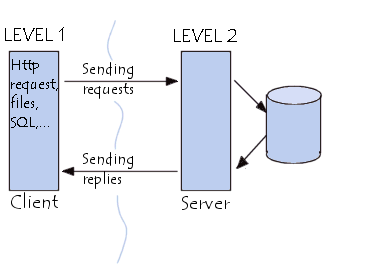
\includegraphics[scale=0.75]{cs-images-2-tier.png}
	\caption{Схема}
	\clearpage
\end{figure}

Здесь четко видно, что есть клиент (1-ый уровень), который позволяет человеку сделать запрос, и есть сервер, который обрабатывает запрос клиента.

Если говорить про многоуровневую архитектуру взаимодействия клиент-сервер, то в качестве примера можно привести любую современную СУБД (за исключением библиотеки SQLite, которая в принципе не использует концепцию клиент-сервер).  Суть многоуровневой архитектуры заключается в том, что запрос клиента обрабатывается сразу несколькими серверами. Такой подход позволяет значительно снизить нагрузку на сервер из-за того, что происходит распределение операций, но в то же самое время данный подход не такой надежный, как двухзвенная архитектура (рисунок 6.2).

\begin{figure}[h!]
\centering
	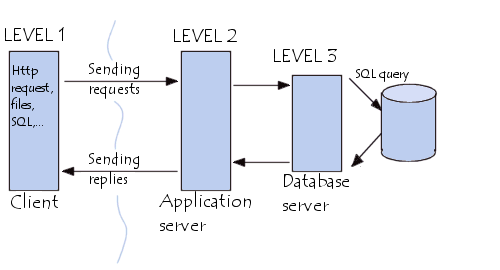
\includegraphics[scale=0.75]{cs-images-3-tier.png}
	\caption{Схема}
	\clearpage
\end{figure}

Типичный пример трехуровневой модели клиент-сервер. Если говорить в контексте систем управления базами данных, то первый уровень – это клиент, который позволяет нам писать различные SQL запросы к базе данных. Второй уровень – это движок СУБД, который интерпретирует запросы и реализует взаимодействие между клиентом и файловой системой, а третий уровень – это хранилище данных.

Если мы посмотрим на данную архитектуру с позиции сайта. То первый уровень можно считать браузером, с помощью которого посетитель заходит на сайт, второй уровень – это связка Nginx + Node, а третий уровень – это база данных. 

Главным преимуществом модели клиент-сервер является то, что код клиента и сервера разделен. Все высоконагруженные вычисления происходят на мощный серверах, а клиентская машина, к которым предъявляются менее серьезные требования, не несет большой нагрузки.

Учьтя всё вышесказанное можно смоделировать клиент-серверную структуру для нашего приложения. Она будут представлена трехуровневой системой. В добавок к ней главный сервер веб-приложения будет связан не только с сервером базы данных, но и с серверами пользователей, которые предоставляют api с данными для своих систем воддельности. 
